\documentclass{standalone}
\usepackage{tikz}
\usetikzlibrary{patterns, positioning}

\begin{document}
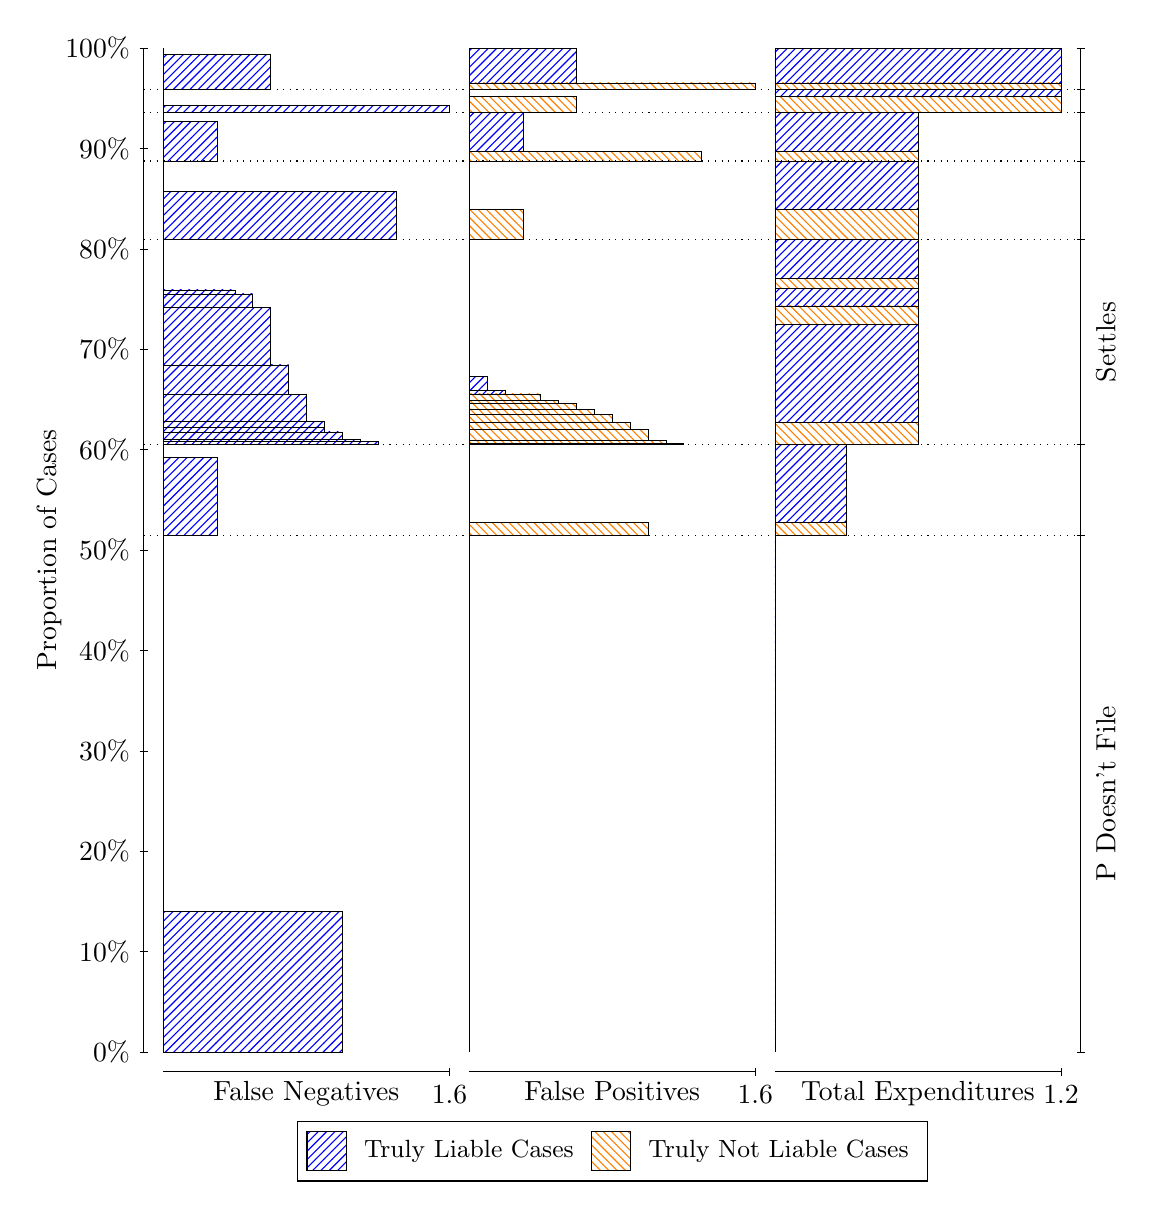
\begin{tikzpicture}
\draw[black, very thin] (1.5,1.75) -- (1.5,14.5);
\node[rotate=90, anchor=center] at (0.3, 8.125) {Proportion of Cases};
\draw[black, very thin] (1.45,1.75) -- (1.55,1.75);
\node[anchor=east] at (1.45, 1.75) {0\%};
\draw[black, very thin] (1.45,3.025) -- (1.55,3.025);
\node[anchor=east] at (1.45, 3.025) {10\%};
\draw[black, very thin] (1.45,4.3) -- (1.55,4.3);
\node[anchor=east] at (1.45, 4.3) {20\%};
\draw[black, very thin] (1.45,5.575) -- (1.55,5.575);
\node[anchor=east] at (1.45, 5.575) {30\%};
\draw[black, very thin] (1.45,6.85) -- (1.55,6.85);
\node[anchor=east] at (1.45, 6.85) {40\%};
\draw[black, very thin] (1.45,8.125) -- (1.55,8.125);
\node[anchor=east] at (1.45, 8.125) {50\%};
\draw[black, very thin] (1.45,9.4) -- (1.55,9.4);
\node[anchor=east] at (1.45, 9.4) {60\%};
\draw[black, very thin] (1.45,10.675) -- (1.55,10.675);
\node[anchor=east] at (1.45, 10.675) {70\%};
\draw[black, very thin] (1.45,11.95) -- (1.55,11.95);
\node[anchor=east] at (1.45, 11.95) {80\%};
\draw[black, very thin] (1.45,13.225) -- (1.55,13.225);
\node[anchor=east] at (1.45, 13.225) {90\%};
\draw[black, very thin] (1.45,14.5) -- (1.55,14.5);
\node[anchor=east] at (1.45, 14.5) {100\%};

\draw[black, very thin] (13.4,1.75) -- (13.4,14.5);
\draw[black, very thin] (13.35,1.75) -- (13.45,1.75);
\node[anchor=west] at (13.35, 1.75) {};
\draw[black, very thin] (13.35,8.311) -- (13.45,8.311);
\node[anchor=west] at (13.35, 8.311) {};
\draw[black, very thin] (13.35,9.4646) -- (13.45,9.4646);
\node[anchor=west] at (13.35, 9.4646) {};
\draw[black, very thin] (13.35,12.07) -- (13.45,12.07);
\node[anchor=west] at (13.35, 12.07) {};
\draw[black, very thin] (13.35,13.065) -- (13.45,13.065);
\node[anchor=west] at (13.35, 13.065) {};
\draw[black, very thin] (13.35,13.686) -- (13.45,13.686);
\node[anchor=west] at (13.35, 13.686) {};
\draw[black, very thin] (13.35,13.972) -- (13.45,13.972);
\node[anchor=west] at (13.35, 13.972) {};
\draw[black, very thin] (13.35,14.5) -- (13.45,14.5);
\node[anchor=west] at (13.35, 14.5) {};

\draw[black, very thin, pattern color=blue, pattern=north east lines] (1.75,1.75) rectangle (4.0208,3.5337);
\draw[black, very thin, pattern color=orange, pattern=north west lines] (1.75,3.5337) rectangle (1.75,8.311);
\draw[black, very thin, pattern color=blue, pattern=north east lines] (1.75,8.311) rectangle (2.4312,9.2977);
\draw[black, very thin, pattern color=orange, pattern=north west lines] (1.75,9.2977) rectangle (1.75,9.4646);
\draw[black, very thin, pattern color=blue, pattern=north east lines] (1.75,9.4646) rectangle (4.475,9.4996);
\draw[black, very thin, pattern color=blue, pattern=north east lines] (1.75,9.4996) rectangle (4.2479,9.5317);
\draw[black, very thin, pattern color=blue, pattern=north east lines] (1.75,9.5317) rectangle (4.0208,9.6252);
\draw[black, very thin, pattern color=blue, pattern=north east lines] (1.75,9.6252) rectangle (3.7937,9.6899);
\draw[black, very thin, pattern color=blue, pattern=north east lines] (1.75,9.6899) rectangle (3.7937,9.761);
\draw[black, very thin, pattern color=blue, pattern=north east lines] (1.75,9.761) rectangle (3.5667,10.106);
\draw[black, very thin, pattern color=blue, pattern=north east lines] (1.75,10.106) rectangle (3.3396,10.477);
\draw[black, very thin, pattern color=blue, pattern=north east lines] (1.75,10.477) rectangle (3.1125,11.202);
\draw[black, very thin, pattern color=blue, pattern=north east lines] (1.75,11.202) rectangle (2.8854,11.378);
\draw[black, very thin, pattern color=blue, pattern=north east lines] (1.75,11.378) rectangle (2.6583,11.427);
\draw[black, very thin, pattern color=orange, pattern=north west lines] (1.75,11.427) rectangle (1.75,12.07);
\draw[black, very thin, pattern color=blue, pattern=north east lines] (1.75,12.07) rectangle (4.7021,12.683);
\draw[black, very thin, pattern color=orange, pattern=north west lines] (1.75,12.683) rectangle (1.75,13.065);
\draw[black, very thin, pattern color=blue, pattern=north east lines] (1.75,13.065) rectangle (2.4312,13.568);
\draw[black, very thin, pattern color=orange, pattern=north west lines] (1.75,13.568) rectangle (1.75,13.686);
\draw[black, very thin, pattern color=blue, pattern=north east lines] (1.75,13.686) rectangle (5.3833,13.769);
\draw[black, very thin, pattern color=orange, pattern=north west lines] (1.75,13.769) rectangle (1.75,13.972);
\draw[black, very thin, pattern color=blue, pattern=north east lines] (1.75,13.972) rectangle (3.1125,14.416);
\draw[black, very thin, pattern color=orange, pattern=north west lines] (1.75,14.416) rectangle (1.75,14.5);
\draw[black, very thin, pattern color=orange, pattern=north west lines] (5.6333,1.75) rectangle (5.6333,6.5273);
\draw[black, very thin, pattern color=blue, pattern=north east lines] (5.6333,6.5273) rectangle (5.6333,8.311);
\draw[black, very thin, pattern color=orange, pattern=north west lines] (5.6333,8.311) rectangle (7.9042,8.4779);
\draw[black, very thin, pattern color=blue, pattern=north east lines] (5.6333,8.4779) rectangle (5.6333,9.4646);
\draw[black, very thin, pattern color=orange, pattern=north west lines] (5.6333,9.4646) rectangle (8.3583,9.4771);
\draw[black, very thin, pattern color=orange, pattern=north west lines] (5.6333,9.4771) rectangle (8.1313,9.5136);
\draw[black, very thin, pattern color=orange, pattern=north west lines] (5.6333,9.5136) rectangle (7.9042,9.6566);
\draw[black, very thin, pattern color=orange, pattern=north west lines] (5.6333,9.6566) rectangle (7.6771,9.7446);
\draw[black, very thin, pattern color=orange, pattern=north west lines] (5.6333,9.7446) rectangle (7.45,9.8472);
\draw[black, very thin, pattern color=orange, pattern=north west lines] (5.6333,9.8472) rectangle (7.2229,9.9071);
\draw[black, very thin, pattern color=orange, pattern=north west lines] (5.6333,9.9071) rectangle (6.9958,9.9835);
\draw[black, very thin, pattern color=orange, pattern=north west lines] (5.6333,9.9835) rectangle (6.7687,10.027);
\draw[black, very thin, pattern color=orange, pattern=north west lines] (5.6333,10.027) rectangle (6.5417,10.108);
\draw[black, very thin, pattern color=blue, pattern=north east lines] (5.6333,10.108) rectangle (6.0875,10.156);
\draw[black, very thin, pattern color=blue, pattern=north east lines] (5.6333,10.156) rectangle (5.8604,10.333);
\draw[black, very thin, pattern color=blue, pattern=north east lines] (5.6333,10.333) rectangle (5.6333,12.07);
\draw[black, very thin, pattern color=orange, pattern=north west lines] (5.6333,12.07) rectangle (6.3146,12.452);
\draw[black, very thin, pattern color=blue, pattern=north east lines] (5.6333,12.452) rectangle (5.6333,13.065);
\draw[black, very thin, pattern color=orange, pattern=north west lines] (5.6333,13.065) rectangle (8.5854,13.184);
\draw[black, very thin, pattern color=blue, pattern=north east lines] (5.6333,13.184) rectangle (6.3146,13.686);
\draw[black, very thin, pattern color=orange, pattern=north west lines] (5.6333,13.686) rectangle (6.9958,13.889);
\draw[black, very thin, pattern color=blue, pattern=north east lines] (5.6333,13.889) rectangle (5.6333,13.972);
\draw[black, very thin, pattern color=orange, pattern=north west lines] (5.6333,13.972) rectangle (9.2667,14.056);
\draw[black, very thin, pattern color=blue, pattern=north east lines] (5.6333,14.056) rectangle (6.9958,14.5);
\draw[black, very thin, pattern color=orange, pattern=north west lines] (9.5167,1.75) rectangle (9.5167,6.5273);
\draw[black, very thin, pattern color=blue, pattern=north east lines] (9.5167,6.5273) rectangle (9.5167,8.311);
\draw[black, very thin, pattern color=orange, pattern=north west lines] (9.5167,8.311) rectangle (10.425,8.4779);
\draw[black, very thin, pattern color=blue, pattern=north east lines] (9.5167,8.4779) rectangle (10.425,9.4646);
\draw[black, very thin, pattern color=orange, pattern=north west lines] (9.5167,9.4646) rectangle (11.333,9.7468);
\draw[black, very thin, pattern color=blue, pattern=north east lines] (9.5167,9.7468) rectangle (11.333,10.993);
\draw[black, very thin, pattern color=orange, pattern=north west lines] (9.5167,10.993) rectangle (11.333,11.224);
\draw[black, very thin, pattern color=blue, pattern=north east lines] (9.5167,11.224) rectangle (11.333,11.45);
\draw[black, very thin, pattern color=orange, pattern=north west lines] (9.5167,11.45) rectangle (11.333,11.579);
\draw[black, very thin, pattern color=blue, pattern=north east lines] (9.5167,11.579) rectangle (11.333,12.07);
\draw[black, very thin, pattern color=orange, pattern=north west lines] (9.5167,12.07) rectangle (11.333,12.452);
\draw[black, very thin, pattern color=blue, pattern=north east lines] (9.5167,12.452) rectangle (11.333,13.065);
\draw[black, very thin, pattern color=orange, pattern=north west lines] (9.5167,13.065) rectangle (11.333,13.184);
\draw[black, very thin, pattern color=blue, pattern=north east lines] (9.5167,13.184) rectangle (11.333,13.686);
\draw[black, very thin, pattern color=orange, pattern=north west lines] (9.5167,13.686) rectangle (13.15,13.889);
\draw[black, very thin, pattern color=blue, pattern=north east lines] (9.5167,13.889) rectangle (13.15,13.972);
\draw[black, very thin, pattern color=orange, pattern=north west lines] (9.5167,13.972) rectangle (13.15,14.056);
\draw[black, very thin, pattern color=blue, pattern=north east lines] (9.5167,14.056) rectangle (13.15,14.5);
\draw[black, dotted] (1.5,8.311) -- (13.4,8.311);
\draw[black, dotted] (1.5,9.4646) -- (13.4,9.4646);
\draw[black, dotted] (1.5,12.07) -- (13.4,12.07);
\draw[black, dotted] (1.5,13.065) -- (13.4,13.065);
\draw[black, dotted] (1.5,13.686) -- (13.4,13.686);
\draw[black, dotted] (1.5,13.972) -- (13.4,13.972);
\draw[black, very thin] (1.75,1.5) -- (5.3833,1.5);
\node[anchor=north] at (3.5667, 1.5) {False Negatives};
\draw[black, very thin] (5.3833,1.45) -- (5.3833,1.55);
\node[anchor=north] at (5.3833, 1.45) {1.6};

\draw[black, very thin] (5.6333,1.5) -- (9.2667,1.5);
\node[anchor=north] at (7.45, 1.5) {False Positives};
\draw[black, very thin] (9.2667,1.45) -- (9.2667,1.55);
\node[anchor=north] at (9.2667, 1.45) {1.6};

\draw[black, very thin] (9.5167,1.5) -- (13.15,1.5);
\node[anchor=north] at (11.333, 1.5) {Total Expenditures};
\draw[black, very thin] (13.15,1.45) -- (13.15,1.55);
\node[anchor=north] at (13.15, 1.45) {1.2};

\node[black, centered, rotate=90] at (13.72, 5.0305) {P Doesn't File};

\node[black, centered, rotate=90] at (13.72, 10.767) {Settles};





\draw (7.449999999999999,1.5) node[draw=none] (baseCoordinate) {};
\begin{scope}[align=center]
        \matrix[scale=0.5, draw=black, below=0.5cm of baseCoordinate, nodes={draw}, column sep=0.1cm]{
            \node[rectangle, draw, minimum width=0.5cm, minimum height=0.5cm, pattern=north east lines, pattern color=blue] {}; &
            \node[draw=none, font=\small] (B) {Truly Liable Cases}; &
            \node[rectangle, draw, minimum width=0.5cm, minimum height=0.5cm, pattern=north west lines, pattern color=orange] {}; &
            \node[draw=none, font=\small] (B) {Truly Not Liable Cases}; \\
            };
\end{scope}

\end{tikzpicture}
\end{document}